% Präambel
\documentclass[%
fontsize=12pt,					% Schriftgröße
paper=a4,						% Papierformat
twoside=false, 					% einseitiges (oneside) oder zweiseitiges (twoside) Dokument
listof=totoc, 					% Tabellen- und Abbildungsverzeichnis ins Inhaltsverzeichnis
bibliography=totoc,				% Literaturverzeichnis ins Inhaltsverzeichnis aufnehmen
titlepage, 						% Titlepage-Umgebung statt \maketitle
headsepline, 					% horizontale Linie unter Kolumnentitel
%abstracton,					% Überschrift beim Abstract einschalten, Abstract muss dazu in {abstract}-Umgebung stehen
DIV=12,							% Satzspiegeleinstellung, 12 ist Standar bei KOMA
%BCOR=6mm,						% Bindekorrektur, die den Seitenspiegel um 6mm nach rechts verschiebt,
cleardoublepage=empty,			% Stil einer leeren eingefügten Seite bei Kapitelwechsel
parskip,							% Absatzabstand bei Absatzwechsel einfügen
ngerman
]{scrbook}			
\usepackage[setspace=false]{scrhack}
\usepackage[utf8]{inputenc} 	% ermöglicht die direkte Eingabe von Umlauten
\usepackage[T1]{fontenc} 		% Ausgabe aller zeichen in einer T1-Codierung (wichtig für die Ausgabe von Umlauten!)
\usepackage{babel} 	% deutsche Trennungsregeln und Übersetzung der festcodierten Überschriften
\setlength{\parindent}{0ex} 	% bei neuem Abschnitt nicht einrücken
%------
% Folgende Einstellungen entsprechen den Vorgaben der Leitlinien
\usepackage[onehalfspacing]{setspace}
% Ende Leitlinien
%------
%------
% Folgende Einstellungen sind bei größeren Arbeiten mit viel Text zu empfehlen.
% Hierbei oben DIV=16 einstellen und Zeile \usepackage[onehalfspacing]{setspace} auskommentieren.
%\linespread{1.2}\selectfont     % Zeilenabstand erhöhen - größere Werte als 1.2 nicht verwenden!!
% Ende Einstellung große Arbeiten mit viel Text.
%------------------------------------------------------------------------------------
\usepackage{comment}			% mir    % zum blockweisen auskommentieren
%------------------------------------------------------------------------------------
% Tabellenpackete
\usepackage{tabularx}			% mir    % Zum erstellen von Tabellen, die ihre Größe anpassen
\usepackage{longtable}			% mir	 % Tabellen über mehrere Seiten möglich
\usepackage{adjustbox}			% mir
\usepackage{array}				% mir

%------------------------------------------------------------------------------------
% PDF Layout
\usepackage{geometry}			% mir
%------------------------------------------------------------------------------------
% Zum ermöglichen, dass Dinge ganz am Schluss manuell platziert werden
\usepackage{afterpage}			% mir
%------------------------------------------------------------------------------------
\usepackage{siunitx}			% Vereinfachte Eingabe von Einheiten in Formeln
\sisetup{
	number-unit-product = \;,
	inter-unit-product = \:,
	exponent-product = \cdot,
	output-decimal-marker = {,}
}
\usepackage{wrapfig}
\usepackage{float}
\usepackage{graphicx}  			% Einbinden von Grafiken erlauben
\usepackage[format=hang,		% Formatierungen von Unter- / Überschriften
font=normal,
labelfont=bf,
justification=RaggedRight,
singlelinecheck=true,
aboveskip=1mm
]{caption}
% ------------------------------------------------------------------------------------------
% GANTT-CHART-Diagramm Spezifisches:
\usepackage{pgfgantt}
\definecolor{barblue}{RGB}{153,204,254}
\definecolor{groupblue}{RGB}{51,102,254}
\definecolor{linkred}{RGB}{165,0,33}
\definecolor{absentcolor}{RGB}{0,200,200}
\setganttlinklabel{s-s}{START-ZU-START}
\setganttlinklabel{f-s}{ENDE-ZU-START}
\setganttlinklabel{f-f}{ENDE-ZU-ENDE}
% ------------------------------------------------------------------------------------------
% ------------------------------------------------------------------------------------------
%%%%Literatureinbindung mit Biber

\usepackage[backend=biber, %% Hilfsprogramm "biber" beim Compilieren nutzen (statt "biblatex" oder "bibtex")
style=numeric, %% Zitierstil (siehe Dokumentation) alternativ "alphabetic" bei Zitirschlüssel
natbib=true, %% Bereitstellen von natbib-kompatiblen Zitierkommandos
hyperref=true, %% hyperref-Paket verwenden, um Links zu erstellen
sorting=none, %% Zitate in der Reihenfolge ihres Auftretens im Text anzeigen (Eingefügt 18.04.24)
]{biblatex}
\setcounter{biburllcpenalty}{7000}
\setcounter{biburlucpenalty}{8000}



% \addbibresource{literature/literatur1.bib} %% Einbinden der bib-Datei. Endung .bib unbedingt ergänzen
%\addbibresource{literature/literatur2.bib} %% Einbinden mehrerer bib-Dateien mit zusätzlichem \addbibresource - Befehl----------------------beiden oberen aus Vorlage

% ------------------------------------------------------------------------------------------
% ------------------------------------------------------------------------------------------
\usepackage{csquotes}

% Neue Zeilen hinzufügen, um das Zugriffsdatum anzuzeigen
\DeclareLabeldate{				% von mir
	\field{urldate}				% von mir
}								% von mir

% Folgende Zeilen sind auszukommentieren, falls runde Klammern und ein vgl. bei Zitaten erscheinen sollen.
%\makeatletter
%\renewcommand{\@cite}[2]{(vgl. {#1\if@tempswa , #2\fi})} 
%\renewcommand{\@biblabel}[1]{(#1)}
%\makeatother

\usepackage{pdfpages}

\usepackage{enumitem}			% Erlaubt Änderung der Nummerierung in der Umgebung enumerate

\usepackage{amsmath}			% Ergänzungen für Formeln
\usepackage{textcomp} 			% zum Einsatz von Eurozeichen u. a. Symbolen
\usepackage{eurosym}			% bessere Darstellung Euro-Symbol mit \euro

\usepackage[					% Einstellunge Paket hyperref
hyperfootnotes=false,			% im pfd-Output Fußnoten nicht verlinken
hidelinks						% Entfernen von farbigen Umrandungen der Links
]{hyperref}

\usepackage{makeidx}			% Paket zur Erstellung eines Index
\usepackage[intoc]{nomencl} 	% zur Erstellung des Abkürzungsberzeichnisses

\usepackage[					% Einstellungen für Fußnoten
bottom,							% Ausrichtung unten
multiple,						% Trennung durch Seperator bei mehreren Fußnoten
hang,
marginal
]{footmisc}

\usepackage{calc}				% Paket zum Berechnen von Längen z.B. 0.8\linewidth
\usepackage{subcaption}			% hinzugefügt von mir, ermöglicht 2x2 Matrix mit Bildern

\usepackage{xcolor} 			% einfache Verwendung von Farben in nahezu allen Farbmodellen

\usepackage{listings}			% Darstellung von Quellcode mit den Umgebungen {lstlisting}, \lstinline und \lstinputlisting
\lstset{literate=				% Damit können Umlaute innerhalb Listings geschrieben werden
	{Ö}{{\"O}}1
	{Ä}{{\"A}}1
	{Ü}{{\"U}}1
	{ß}{{\ss}}1
	{ü}{{\"u}}1
	{ä}{{\"a}}1
	{ö}{{\"o}}1
}
\definecolor{mygreen}{rgb}{0,0.6,0}
\definecolor{mygray}{rgb}{0.5,0.5,0.5}
\definecolor{mymauve}{rgb}{0.58,0,0.82}
\lstset{ %
	backgroundcolor=\color{white},   % choose the background color; you must add \usepackage{color} or \usepackage{xcolor}; should come as last argument
	basicstyle=\footnotesize,        % the size of the fonts that are used for the code
	breakatwhitespace=false,         % sets if automatic breaks should only happen at whitespace
	breaklines=true,                 % sets automatic line breaking
	captionpos=t,                    % sets the caption-position to (b) bottom or (t) top
	commentstyle=\color{mygreen},    % comment style
	deletekeywords={...},            % if you want to delete keywords from the given language
	escapeinside={\%*}{*)},          % if you want to add LaTeX within your code
	escapeinside={(*@}{@*)},
	extendedchars=true,              % lets you use non-ASCII characters; for 8-bits encodings only, does not work with UTF-8
	frame=none,	                   	% "single" adds a frame around the code; "none"
	keepspaces=true,                 % keeps spaces in text, useful for keeping indentation of code (possibly needs columns=flexible)
	keywordstyle=\color{blue},       % keyword style
	language=[LaTeX]TeX,             % the language of the code
	morekeywords={*,nomenclature},   % if you want to add more keywords to the set
	numbers=left,                    % where to put the line-numbers; possible values are (none, left, right)
	numbersep=5pt,                   % how far the line-numbers are from the code
	numberstyle=\tiny\color{mygray}, % the style that is used for the line-numbers
	rulecolor=\color{black},         % if not set, the frame-color may be changed on line-breaks within not-black text (e.g. comments (green here))
	showspaces=false,                % show spaces everywhere adding particular underscores; it overrides 'showstringspaces'
	showstringspaces=false,          % underline spaces within strings only
	showtabs=false,                  % show tabs within strings adding particular underscores
	stepnumber=1,                    % the step between two line-numbers. If it's 1, each line will be numbered
	stringstyle=\color{mymauve},     % string literal style
	tabsize=2,	                   % sets default tabsize to 2 spaces
	title=\lstname                   % show the filename of files included with \lstinputlisting; also try caption instead of title
}

\makeindex						% Indexverzeichnis erstellen
\makenomenclature				% Abkürzungsverzeichnis erstellen
%------------------------------------------------------------------------------------
%------------------------------------------------------------------------------------

% To Access Codeimplementation: (26.04.2024)
\definecolor{vscode-blue}{RGB}{0, 122, 204}
\definecolor{vscode-darkblue}{RGB}{0, 60, 120}
\definecolor{vscode-green}{RGB}{86, 156, 34}
\definecolor{vscode-yellow}{RGB}{209, 154, 102}
\definecolor{vscode-red}{RGB}{204, 24, 30}
\definecolor{vscode-gray}{RGB}{128, 128, 128}
\definecolor{vscode-darkgray}{RGB}{40, 42, 46}
\definecolor{vscode-lightgray}{RGB}{197, 200, 198}
\definecolor{vscode-darkgreen}{RGB}{35, 138, 115}
\definecolor{vscode-orange}{RGB}{255, 121, 198}
\definecolor{vscode-brown}{RGB}{139, 69, 19}
\definecolor{vscode-purple}{RGB}{128, 0, 128}
% S 26.04.2024
% Definiere die Sprache Batch
\lstdefinelanguage{batch}{
	keywords={@echo, echo, pause, cd, start, timeout, rem, powershell, nul, python},
	sensitive=false,
	morecomment=[l]{rem\ },
	morestring=[b]",
}
% Definiere die Sprache CMake
\lstdefinelanguage{cmake}{
	keywords={add_executable, add_library, add_subdirectory, add_test, cmake_minimum_required, configure_file, file, find_package, get_filename_component, include_directories, include, link_directories, list, message, project, set, target_compile_definitions, target_include_directories, target_link_libraries, target_sources, add_custom_target,add_custom_command, SET, find_program},
	morekeywords=[2]{if, endif},
	morekeywords=[3]{PATHS, DOC, NOT, FATAL_ERROR, OUTPUT, COMMAND, DEPENDS, NAME},
	sensitive=true,
	comment=[l]{\#},
	morestring=[b]",
}

% Definiere den Code-Stil im VS Code-Stil
\lstdefinestyle{CStyle}{
	language=C,
	basicstyle=\small\ttfamily,
	commentstyle=\color{vscode-green},
	keywordstyle=\color{vscode-blue},
	numberstyle=\tiny\color{vscode-gray},
	stringstyle=\color{vscode-orange},
	backgroundcolor=\color{white},
	showspaces=false,
	showstringspaces=false,
	showtabs=false,
	tabsize=2,
	frame=single,
	rulecolor=\color{vscode-lightgray},
	captionpos=b,
	breaklines=true,
	breakatwhitespace=false,
	escapeinside={\%*}{*)},
	numbers=left,
	stepnumber=1,
	numbersep=5pt,
}
\lstdefinestyle{CStyleSmall}{
	language=C,
	basicstyle=\ttfamily\scriptsize,
	commentstyle=\color{vscode-green},
	keywordstyle=\color{vscode-blue},
	keywordstyle=[2]{\color{vscode-darkgreen}},
	numberstyle=\tiny\color{vscode-gray},
	stringstyle=\color{vscode-orange},
	backgroundcolor=\color{white},
	showspaces=false,
	showstringspaces=false,
	showtabs=false,
	tabsize=2,
	frame=single,
	rulecolor=\color{vscode-lightgray},
	captionpos=b,
	breaklines=true,
	breakatwhitespace=false,
	escapeinside={\%*}{*)},
	numbers=left,
	stepnumber=1,
	numbersep=5pt,
	morekeywords=[2]{uint8,uint16,uint32,float32},
}
\lstdefinestyle{BatchStyle}{
	language=batch,
	basicstyle=\small\ttfamily,
	commentstyle=\color{vscode-green},
	keywordstyle=\color{vscode-blue},
	numberstyle=\tiny\color{vscode-gray},
	stringstyle=\color{vscode-brown},
	backgroundcolor=\color{white},
	showspaces=false,
	showstringspaces=false,
	showtabs=false,
	tabsize=2,
	frame=single,
	rulecolor=\color{vscode-lightgray},
	captionpos=b,
	breaklines=true,
	breakatwhitespace=false,
	escapeinside={\%*}{*)},
	numbers=left,
	stepnumber=1,
	numbersep=5pt,
}
\lstdefinestyle{PythonStyle}{
	language=Python,                     % the language of the code
	basicstyle=\ttfamily\scriptsize,     % the size and font of the code
	backgroundcolor=\color{white},       % choose the background color
	commentstyle=\color{vscode-green},   % comment style
	keywordstyle=\color{vscode-blue},    % keyword style
	numberstyle=\tiny\color{vscode-gray},  % the style for line numbers
	stringstyle=\color{vscode-brown},    % string literal style
	breaklines=true,                     % automatic line breaking only at whitespace
	captionpos=b,                        % sets the caption-position to bottom
	tabsize=2,                           % sets default tabsize to 2 spaces
	frame=single,                        % adds a frame around the code
	rulecolor=\color{black},             % if not set, the frame-color may be changed on line-breaks within not-black text (e.g. comments (green here))
	showspaces=false,                    % show spaces everywhere adding particular underscores; it overrides 'showstringspaces'
	showstringspaces=false,              % underline spaces within strings only
	showtabs=false,                      % show tabs within strings adding particular underscores
	title=\lstname,                      % show the filename of files included with \lstinputlisting; also try caption instead of title
	escapeinside={\%*}{*)},              % if you want to add LaTeX within your code
	morekeywords={*,...},                 % if you want to add more keywords to the set
	deletekeywords={...}                 % if you want to delete keywords from the given language
}
\lstdefinestyle{PythonStyleBig}{
	language=Python,                     % the language of the code
	basicstyle=\small\ttfamily,          % the size and font of the code
	backgroundcolor=\color{white},       % choose the background color
	commentstyle=\color{vscode-green},   % comment style
	keywordstyle=\color{vscode-blue},    % keyword style
	numberstyle=\tiny\color{vscode-gray},  % the style for line numbers
	stringstyle=\color{vscode-brown},    % string literal style
	breaklines=true,                     % automatic line breaking only at whitespace
	captionpos=b,                        % sets the caption-position to bottom
	tabsize=2,                           % sets default tabsize to 2 spaces
	frame=single,                        % adds a frame around the code
	rulecolor=\color{black},             % if not set, the frame-color may be changed on line-breaks within not-black text (e.g. comments (green here))
	showspaces=false,                    % show spaces everywhere adding particular underscores; it overrides 'showstringspaces'
	showstringspaces=false,              % underline spaces within strings only
	showtabs=false,                      % show tabs within strings adding particular underscores
	title=\lstname,                      % show the filename of files included with \lstinputlisting; also try caption instead of title
	escapeinside={\%*}{*)},              % if you want to add LaTeX within your code
	morekeywords={*,...},                 % if you want to add more keywords to the set
	deletekeywords={...}                 % if you want to delete keywords from the given language
}
\lstdefinestyle{CMakeStyle}{
	language=CMake,
	basicstyle=\ttfamily\scriptsize,
	commentstyle=\color{vscode-green},
	keywordstyle=\color{vscode-blue},
	keywordstyle=[2]{\color{vscode-purple}},
	keywordstyle=[3]{\color{vscode-darkblue}},
	numberstyle=\tiny\color{vscode-gray},
	stringstyle=\color{vscode-orange},
	backgroundcolor=\color{white},
	showspaces=false,
	showstringspaces=false,
	showtabs=false,
	tabsize=2,
	frame=single,
	rulecolor=\color{vscode-lightgray},
	captionpos=b,
	breaklines=true,
	breakatwhitespace=false,
	escapeinside={\%*}{*)},
	numbers=left,
	stepnumber=1,
	numbersep=5pt,
}
% Änderung der Bezeichnung für Listings
\renewcommand{\lstlistingname}{Aufzählung} % 19.06.2024
\renewcommand{\lstlistlistingname}{Aufzählungen} % 19.06.2024
%------------------------------------------------------------------------------------ 
%------------------------------------------------------------------------------------ 
% Zum Aktualisieren des Abkürzungsverzeichnisses (Nomenklatur) bitte auf der Kommandozeile folgenden Befehl aufrufen : im Terminal
% makeindex <Dateiname>.nlo -s nomencl.ist -o <Dateiname>.nls
%%%%%%%%%% hier: 
% für Simon
% cd C:\Users\schaeffs\OneDrive - Webasto Group\Dokumente\02_Theoriephasen_an_der_DHBW\05_Semester\01_Studienarbeit_T3_3100\T3_3100\latex_doku_master
%
% makeindex WissBer_PA_SA_BA.nlo -s nomencl.ist -o WissBer_PA_SA_BA.nls
%%%%%%%%%%
% Oder besser: Kann in TexStudio unter Tools-Benutzer als Shortlink angelegt werden
% Konfiguration unter: Optionen-Erzeugen-Benutzerbefehle: makeindex -s nomencl.ist -t %.nlg -o %.nls %.nlo
% -----------------------------------------------------------------------------------------------------------------

% Hier die persönlichen Daten eingeben:

\newcommand{\titel}{Entwicklung eines TIA-Projektes}
\newcommand{\untertitel}{}
\newcommand{\arbeit}{Hausarbeit Industrielle Bussysteme}
\newcommand{\studiengang}{Elektrotechnik}
\newcommand{\studienrichtung}{Automation}
\newcommand{\studienschwerpunkt}{}
\newcommand{\autorone}{Simon Schäffler}
\newcommand{\autortwo}{Alexander Drexl}
\newcommand{\autorthree}{Florian Prumbs}
\newcommand{\matrikelnrone}{5710369}
\newcommand{\matrikelnrtwo}{3982016}
\newcommand{\matrikelnrthree}{1848162}
\newcommand{\kurs}{FN -TEA22}
\newcommand{\firma}{Webasto Roof \& Components SE}
\newcommand{\abgabe}{\today}
\newcommand{\betreuerdhbw}{Prof. Dr.-Ing Thorsten Kever}
\newcommand{\betreuerfirma}{nobody}
\newcommand{\jahr}{2024}% für Angabe im Copyright-Vermerk der Titelseite
\newcommand{\city}{Friedrichshafen}

% Folgende Zeilen definieren Abkürzungen, um Befehle schneller eingeben zu können
\newcommand{\ua}{\mbox{u.\,a.\ }}
\newcommand{\zB}{\mbox{z.\,B.\ }}
\newcommand{\bs}{$\backslash$}
\newcommand*\diff{\mathop{}\!\mathrm{d}}	% Differentialzeichen
\newcommand*\Diff[1]{\mathop{}\!\mathrm{d^#1}} % Differentialzeichen höherer Ableitung
\newcommand*\jj{\mathop{}\!\mathrm{j}}	% Komplexe Zahl j

% Folgende Zeilen weden benötigt, um Tikz und PGF-Plot-Grafiken einzubinden
\usepackage{pgfplots}
\usepackage{pgfplotstable}
\pgfplotsset{compat=newest,width=0.6\linewidth}
\usepgfplotslibrary{smithchart}
\usepackage{tikz}						% Tikz sollte nach Listings Pakete geladen werden.
% \usetikzlibrary{arrows}
\usetikzlibrary{arrows.meta, decorations.pathreplacing, shapes, positioning, patterns}
\hyphenation{Schrift-ar-ten}

\DeclareRobustCommand{\_}{\allowbreak\string_} % Erlaubt Zeilenumbrüche bei Symbol ''_''

% -------------------------------------------------------------------------------------------
%                     Beginn des Dokumenteninhalts
% -------------------------------------------------------------------------------------------
\begin{document}
\let\texteuro\euro						% Eingabe \texteuro, € oder \euro erzeugt gleiches Ergebnis
\setcounter{secnumdepth}{3}				% Nummerierungstiefe fürs Inhaltsverzeichnis
\setcounter{tocdepth}{3}
\sffamily								% für die Titelei serifenlose Schrift verwenden

% ------------------------------ Titelei -----------------------------------------------------

\thispagestyle{plain}
\hypersetup{pageanchor=false}
\begin{titlepage}
\enlargethispage{4.0cm}
\sffamily 								% Serifenlose Grundschrift für die Titelseite einstellen

\parbox{0.5\linewidth}{
\begin{flushleft}

\includegraphics[width=0.6\linewidth]{images/Webasto_Logo.png}
\end{flushleft}
}
\parbox{0.5\linewidth}{
\begin{flushright}
	
\includegraphics[width=0.6\linewidth]{images/DHBW_d_R_FN_46mm_4c}
	\\[5ex]
\end{flushright}
}
				

\begin{center}

{\fontsize{25.84pt}{17pt}\selectfont
\textbf{\titel}\\[1.5ex]}
{\fontsize{14pt}{17pt}\selectfont
\textbf{\untertitel}\\[5ex]}
{\fontsize{17pt}{20pt}\selectfont
\textbf{\arbeit}\\[2ex]}
{\fontsize{14pt}{17pt}\selectfont
Studiengang \studiengang\\[2ex]}
{\fontsize{12pt}{14pt}\selectfont
Studienrichtung \studienrichtung\\[1ex]
Duale Hochschule Baden-Württemberg Ravensburg, Campus Friedrichshafen\\[5ex]
von\\[1ex]
\autorone,~\autortwo~und~\autorthree \\[15ex]}


\end{center}

\begin{flushleft}
{\fontsize{12pt}{14pt}\selectfont
\begin{tabular}{ll}
Abgabedatum:					& \quad \abgabe \\
Bearbeitungszeitraum:		   	& \quad 15.11.2024 - 06.12.2024 \\ 
Matrikelnummer \autorone: 		& \quad \matrikelnrone \\ 
Martikelnummer \autortwo:		& \quad \matrikelnrtwo \\
Martikelnummer \autorthree:		& \quad \matrikelnrthree \\
Kurs: 							& \quad \kurs \\
Ausbildungsfirma:	 			& \quad \firma \\ 
% Betreuer der Ausbildungsfirma:  & \quad \betreuerfirma \\ 

\end{tabular}
}
\end{flushleft}
%--------------------------------------------------------------------------------------
%%%%% Nachfolgende Zeilen einkommentieren, wenn Copyrightvermerk gewünscht ist
%\begin{flushleft}
%{\fontsize{11pt}{13pt}\selectfont
%Copyrightvermerk:\\
%Dieses Werk einschließlich seiner Teile ist \textbf{urheberrechtlich geschützt}. Jede Verwertung außerhalb der engen Grenzen des Urheberrechtgesetzes ist ohne Zustimmung des Autors unzulässig und strafbar. Das gilt insbesondere für Vervielfältigungen, Übersetzungen, Mikroverfilmungen sowie die Einspeicherung und Verarbeitung in elektronischen Systemen.
%}
%\end{flushleft}
%\begin{flushright}
%{\fontsize{11pt}{13pt}\selectfont \copyright{} \jahr }
%\end{flushright}
%--------------------------------------------------------------------------------------
\end{titlepage}

\cleardoublepage
\hypersetup{pageanchor=true}
 				% erzeugt die Titelseite
\pagenumbering{roman}					% kleine, römische Seitenzahlen für Titelei
% Ggf. folgende Zeile auskommentieren, falls der Sperrvermerk gewünscht ist.
\begin{comment}
\chapter*{Sperrvermerk} %*-Variante sorgt dafür, das der Sperrvermerk nicht im Inhaltsverzeichnis auftaucht
gemäß Ziffer 1.1.13 der Anlage 1 zu §§ 3, 4 und 5  der Studien- und Prüfungsordnung für die Bachelorstudiengänge im Studienbereich Technik der Dualen Hochschule Baden-Württemberg vom 29.09.2017 in der Fassung vom 25.07.2018:

Der Inhalt dieser Arbeit darf weder als Ganzes noch in Auszügen Personen außerhalb des Prüfungsprozesses und des Evaluationsverfahrens zugänglich gemacht werden, sofern keine anders lautende Genehmigung vom Dualen Partner vorliegt.\\[4ex]

\city, den \today \\[1ex]

\makebox[7cm]{\rule[-0.2cm]{7cm}{0.5pt}} \hfill \makebox[7cm]{\rule[-0.2cm]{7cm}{0.5pt}} \\ % Die Linien
\makebox[7cm]{\autorone} \hfill \makebox[7cm]{\autortwo} \\[10ex] % Die Namen mittig unter den Linien
\end{comment}
\chapter*{Erklärung} %*-Variante sorgt dafür, dass die Erklärung nicht im Inhaltsverzeichnis auftaucht

gemäß Ziffer 1.1.13 der Anlage 1 zu §§ 3, 4 und 5  der Studien- und Prüfungsordnung für die Bachelorstudiengänge im Studienbereich Technik der Dualen Hochschule Baden-Württemberg vom 29.09.2017 in der Fassung vom 25.07.2018.

Wir versichern hiermit, dass unsere Hausarbeit mit dem Thema:
\begin{comment}
Richtiges Auswählen:
Ich versichere hiermit, dass ich meine Bachelorarbeit (bzw. Projektarbeit oder Studienarbeit bzw. Hausarbeit) mit dem Thema:
\end{comment}
\begin{quote}
	\textit{\titel}\textit{ \untertitel }
\end{quote}

selbstständig verfasst und keine anderen als die angegebenen Quellen und Hilfsmittel benutzt wurden.\\[1ex]

\city, den \today \\[1ex]

\makebox[7cm]{\rule[-0.2cm]{7cm}{0.5pt}}\\
\makebox[7cm]{\autorone}\\[2ex]
\makebox[7cm]{\rule[-0.2cm]{7cm}{0.5pt}}\\
\makebox[7cm]{\autortwo}\\[2ex]
\makebox[7cm]{\rule[-0.2cm]{7cm}{0.5pt}}\\
\makebox[7cm]{\autorthree}\\

\rmfamily

\thispagestyle{empty}

\cleardoublepage

 				% Einbinden der eidestattlichen Erklärung
%% is not in WissBer_PA_SA_BA.tex included
\chapter*{Kurzfassung}

\newpage
\chapter*{Abstract}

\cleardoublepage   			% Einbinden des Abstracts

%\tableofcontents						% Erzeugen des Inhalsverzeichnisses
\cleardoublepage


% --------------------------------------------------------------------------------------------
%                    Inhalt der Bachelorarbeit
%---------------------------------------------------------------------------------------------
\pagenumbering{arabic}					% arabische Seitenzahlen für den Hauptteil

\rmfamily

%\chapter{Einleitung}
\label{cha:Einleitung}

%\chapter{Ausgangslage und Herausforderungen}
\label{cha:AusgangslageundHerausforderungen}
werbsfähigkeit des Unternehmens.
\chapter*{Konzeptentwurf}
\label{cha:Konzeptentwurf}

\section*{State Machine}
\label{sec:State Machine}

\subsection*{Initialzustand}
\label{subsec:Initialzustand}

Das System startet im Initialzustand und wechselt direkt in den sogenannten Idle-Zustand. Im Idle-Zustand sind beide LEDs der Anzeige AC2398 ausgeschaltet. In diesem Zustand kann das System je nach den erkannten Eingaben oder Ereignissen in andere Zustände wechseln. Wenn der grüne Knopf gedrückt wird und kein RFID-Tag erkannt wird, speichert das System die aktuelle Systemzeit und bleibt im Idle-Zustand. Dieser Vorgang wird im Diagramm als "Save Time" bezeichnet.

\subsection*{Tag-Erkennung und Verarbeitung}
\label{subsec:Tag-ErkennungundVerarbeitung}

Wird ein NFC-Tag erkannt und liegt kein Fehlerzustand vor, wechselt das System in den Zustand "Tag Detected Handling". In diesem Zustand blinkt die grüne LED mit einer Frequenz von einer Sekunde, um anzuzeigen, dass ein Tag erkannt wurde. Es gibt zwei mögliche Aktionen, vorausgesetzt, es liegt kein Fehlerzustand vor:

Write Tag Handling: Wenn der grüne Knopf gedrückt wird, während das RFID-Tag erkannt wird und die Systemzeit vorhanden ist, wechselt das System in den Zustand "Write Tag Handling". In diesem Zustand wird die zuvor gespeicherte Systemzeit auf das RFID-Tag geschrieben. Die grüne LED leuchtet dauerhaft, um anzuzeigen, dass der Schreibvorgang erfolgreich abgeschlossen wurde. Sobald das RFID-Tag nicht mehr erkannt wird, kehrt das System in den Idle-Zustand zurück.

Delete Tag Handling: Alternativ kann der rote Knopf gedrückt werden, während das RFID-Tag erkannt wird und kein Fehlerzustand vorliegt. In diesem Fall wechselt das System in den Zustand ''Delete Tag Handling''. Hier werden die gespeicherten Daten des RFID-Tags gelöscht, und beide LEDs leuchten dauerhaft, solange das Tag erkannt wird. Sobald das RFID-Tag nicht mehr erkannt wird, kehrt das System in den Idle-Zustand zurück.

\subsection*{Fehlerbehandlung}
\label{subsec:Fehlerbehandlung}

Wenn während des Prozesses ein Fehlerzustand auftritt, wechselt das System in den Zustand "Error State Handling". In diesem Zustand blinkt die rote LED mit einer Frequenz von einer Sekunde, während die grüne LED ausgeschaltet bleibt, um den Fehler anzuzeigen. Der Fehlerzustand bleibt bestehen, bis die Ursache des Fehlers behoben ist. Anschließend erreicht das System den Finalzustand und der gesamte Ablauf beginnt erneut.
\begin{figure}[h!]
	\centering
	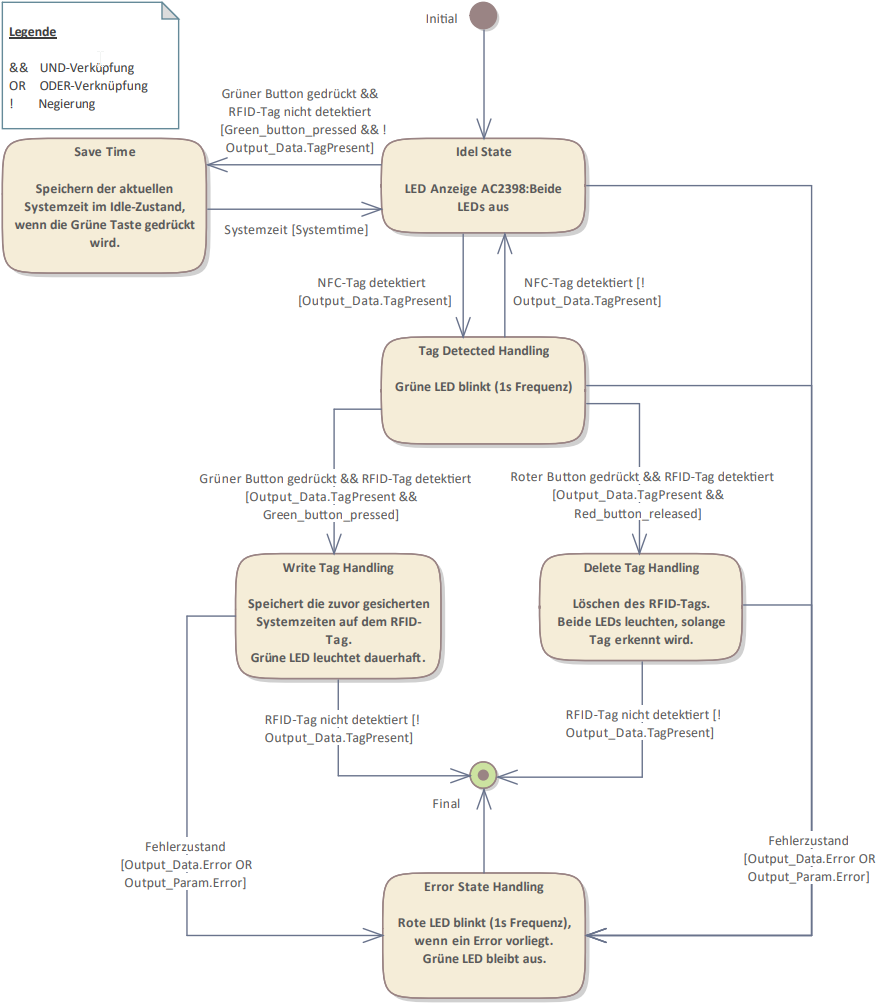
\includegraphics[width=1.0\textwidth]{images/StateMachine.png}
	\vspace{1cm}
	\caption{State-Machine-Diagramm}
	% [Abbildungsverzeichnis]{Bildunterschrift}
	\label{fig:StateMachineDiagramm}
\end{figure}

\clearpage
\newpage
\section*{Variablen-Tabellen}
\label{sec:VariablenTabellen}

Für die verwendete Hardware ''AC2398'' (ein Block mit zwei Tastern, jeweils mit integrierter LED) und das NFC-Modul ''DTI515'' werden die folgenden Variablentabellen (Tabelle \ref{tab:AC2398} und Tabelle \ref{tab:DTI515}) benötigt.

\begin{table}[h!]
	\centering
	\renewcommand{\arraystretch}{1.0} % Verringert den Zeilenabstand
	\footnotesize
	\begin{tabular}{|l|l|l|l|}
		\hline
		\textbf{Name} & \textbf{Datentyp} & \textbf{Adresse} & \textbf{Kommentar}\\ \hline
		RED\_button\_released & Bool & \%I193.2 & 1 wenn roter Taster nicht gedrückt \\ \hline
		Green\_button\_pressed & Bool & \%I193.3 & 1 wenn grüner Taster gedrückt \\ \hline
		Red\_button\_LED\_ON & Bool & \%Q192.0 & wenn 1 dann rote LED vom Taster an \\ \hline
		Green\_button\_LED\_ON & Bool & \%Q192.1 & wenn 1 grüne LED vom Taster an \\ \hline
	\end{tabular}
	\caption{Variablentabelle von AC2398 (Tasterblock)}
	\label{tab:AC2398}
\end{table}
\begin{table}[h!]
	\centering
	\renewcommand{\arraystretch}{1.0} % Verringert den Zeilenabstand
	\footnotesize
	\begin{tabular}{|p{6cm}|p{4.36cm}|p{3cm}|}
		\hline
		\textbf{Name} & \textbf{Datentyp} & \textbf{Adresse} \\ \hline
		Output\_Param.Done & Bool & \%I6.0 \\ \hline
		Output\_Param.Busy & Bool & \%I6.1 \\ \hline
		Output\_Param.Error & Bool & \%I6.2 \\ \hline
		Output\_Param.Status & Word & \%IW8 \\ \hline
		Output\_Param.ExtStatus & DWord & \%ID10 \\ \hline
		Output\_Param.RdValue & UInt & \%IW14 \\ \hline
		Output\_Data.TagPresent & Bool & \%I92.0 \\ \hline
		Output\_Data.Done & Bool & \%I92.1 \\ \hline
		Output\_Data.Busy & Bool & \%I92.2 \\ \hline
		Output\_Data.Error & Bool & \%I92.3 \\ \hline
		Output\_Data.Status & Word & \%IW94 \\ \hline
		Output\_Data.ExStatus & Word & \%IW96 \\ \hline
		Input\_Param.Execute & Bool & \%Q0.0 \\ \hline
		Input\_Param.Mode & UInt & \%QW2 \\ \hline
		Input\_Param.SetValue & UInt & \%QW4 \\ \hline
		Input\_Data.DT\_InAddr & UInt & \%QW16 \\ \hline
		Input\_Data.DT\_OutAddr & UInt & \%QW18 \\ \hline
		Input\_Data.Execute & Bool & \%Q20.0 \\ \hline
		Input\_Data.Force & Bool & \%Q20.1 \\ \hline
		Input\_Data.Mode & UInt & \%QW22 \\ \hline
		Input\_Data.TagMemAddr & UInt & \%QW24 \\ \hline
		Input\_Data.Length & UInt & \%QW26 \\ \hline
		Input\_Data.WrData & Array[0..31] of Byte & \%Q28.0 \\ \hline
		Input\_Data.RdData & Array[0..31] of Byte & \%Q60.0 \\ \hline
	\end{tabular}
	\caption{Variablentabelle von DTI515 (NFC-Modul)}
	\label{tab:DTI515}
\end{table}

Zur Realisierung der in Abbildung \ref{fig:StateMachineDiagramm} dargestellten Logik werden die bausteinlokalen Variablen aus Tabelle \ref{tab:BausteinlokaleVariablen} benötigt. Diese Variablen werden später im Funktionsbaustein ''FB\_RFID\_Manager'' deklariert.

\begin{table}[h!]
	\centering
	\renewcommand{\arraystretch}{1.0} % Verringert den Zeilenabstand
	\footnotesize
	\begin{tabular}{|l|p{1.7cm}|p{5.6cm}|} % p{10cm} sorgt dafür, dass die Kommentare umbrochen werden
		\hline
		\textbf{Name} & \textbf{Datentyp}  & \textbf{Kommentar} \\ \hline
		Tag\_Present & Bool & Wird ein NFC\_Tag erkannt \\ \hline
		Clock1Hz & Bool & Eine Clock mit 1 Herz \\ \hline
		Green\_button & Bool & Wird Grüner Button betätigt \\ \hline
		Red\_button & Bool & Wird Roter Button losgelassen \\ \hline
		Data\_Error & Bool & Fehler im Read/Write Data FBD \\ \hline
		Paramter\_Error & Bool & Fehler im parametrization FBD \\ \hline
		Execute & Bool & Ausführung des Schreibe bzw. Lösch Vorgangs \\ \hline
		Green\_Button\_LED\_State & Bool & Status der LED des grünen Buttons \\ \hline
		Red\_Button\_LED\_State & Bool & Status der LED des roten Buttons \\ \hline
		Data\_Mode & Int & Welcher Modus verwendet wird \\ \hline
		Data\_Write & Array[0..31] of Byte & Eine Liste zum speichern der geschriebenen bzw. gelöschten Bytes \\ \hline
		Data\_Length & Int & Einstellung der Länge der Liste am FBD Read/Write Data \\ \hline
		M1\_Error\_State\_Handling & Bool & Netzwerk 1: Wird ein Fehler erkannt? \\ \hline
		M2\_Error\_State\_Handling\_Clock & Bool & Netzwerk 2: Clock aktiv? \\ \hline
		M3\_Tag\_Detected\_Handling & Bool & Netzwerk 2: Wird ein NFC-Tag erkannt? \\ \hline
		M4\_Tag\_Detected\_Handling\_Clock & Bool & Netzwerk 2: Clock aktiv? \\ \hline
		M5\_Save\_System\_Time & Bool & Netzwerk 3: Wurde einmal die Zeit gespeichert? \\ \hline
		M6\_Write\_Tag\_Handling & Bool & Netzwerk 4: Wird auf den NFC-Tag geschrieben? \\ \hline
		M7\_Delete\_Tag\_Handling & Bool & Netzwerk 5: Wird der NFC-Tag gelöscht \\ \hline
		Green\_LED\_Tag\_Detected\_Handling & Bool & Grüne LED wird eingeschaltet, wenn Tag erkannt wird \\ \hline
		Green\_LED\_Write\_Tag\_Handling & Bool & Grüne LED wird eingeschaltet, wenn NFC-Tag beschrieben wurde \\ \hline
		Green\_LED\_Delete\_Tag\_Handling & Bool & Grüne LED wird eingeschaltet, wenn NFC-Tag gelöscht wurde \\ \hline
		Red\_LED\_Error\_State & Bool & Rote LED wird eingeschaltet, wenn ein Fehlerzustand herrscht \\ \hline
		Systemtime & Bool & Speicher Systemzeit im Format Time \\ \hline
		Systemtimeconv & Bool & Gespeicherte Systemzeit wird Datentyp DInt konvertiert \\ \hline
		Execute\_Write\_Handling & Bool & Ausführung des Schreibbefehls \\ \hline
		Execute\_Delete\_Handling & Bool & Ausführung des Löschbefehls \\ \hline
	\end{tabular}
	\caption{Bausteinlokale Variablen von Funktionsbaustein ''FB\_RFID\_Manager''}
	\label{tab:BausteinlokaleVariablen}
\end{table}

% ------------------------------------------------------------------------------------
%... Text Konzeptentwurf: Gegenüberstellung verschiedener Lösungsansätze und Lösungsgenerierung, etc.
\chapter*{Umsetzung}
\label{cha:Umsetzung}
Im Folgenden soll die Umsetzung der State Machine als SPS-Prpogramm beschrieben werden. Dabei werden die einzelnen Programmbausteine hierarchisch und beginnend beim Organisationsbaustein (OB1) kurz erläutert.

\subsection*{PLC Main}
\label{subsec:PLC_Main}
Im Organisationsbaustein befinden sich in Summe drei Programmbausteine. Dabei handelt es sich um die Bausteine ''DTI515 parametrization'', ''DTI515 Read/Write Data'' und ''DTI515 RFID Manager''. Die ersten beiden Bausteine müssen mit Werten versorgt werden, um die RFID-Antenne zu betreiben.
Der Block DTI515 parametrization bietet drei Eingänge, die für die Umsetzung relevant sind. Die Eingänge heißen ''Mode'', ''SetValue'' und ''Execute''. Mit dem Eingang Mode kann festgelegt werden, ob gelesen oder geschrieben werden soll. An dem Eingang SetValue wird im Schreibfall der Wert, welcher geschrieben wird, übergeben. Mit Execute wird das letztendliche Schreiben oder Lesen getriggert. DTI515 parametrization bietet außerdem insgesamt 6 Ausgänge. Relevant für das Projekt ist nur der Ausgang ''Error'', welcher anzeigt, dass ein Fehler aufgetreten ist. Alle Eingänge und Ausgänge sind mit PLC-Variablen verknüpft.
Der Block DTI515 Read/Write Data hat sieben Eingänge. Vier dieser Eingänge sind für die Umsetzung des Projekts relevant. Diese werden durch PLC-Variablen versorgt, welche vom RFID-Manger gesetzt werden. Es handelt sich um die Eingänge ''Execute'', ''Mode'', ''Length'' und ''WrData''. Mit Mode wird gewählt, ob gelesen oder geschrieben wird. Über Length wird festgelegt, wie viele Byte im Schreibfall geschrieben werden sollen. WrData ist der Eingang, der mit den zu versendenden Daten versorgt wird. Execute triggert das letztendliche Schreiben von Daten auf den RFID-Tag. Von den sechs Ausgängen dieses Bausteins sind 2 relevant. Zum einen der Ausgang ''TagPresent''. Zum anderen der Ausgang ''Error''. Mittels TagPresent kann ermittelt werden. ob sich ein RFID-Tag in der Nähe der Antenne befindet. Error wird überprüft, um festzustellen, ob das Schreiben fehlerfrei verlaufen ist. Der Wert beider wird in einer PLC-Variable abgelegt (siehe Abb. \ref{fig:Main[OB1]Netzwerk1}, \ref{fig:Main[OB1]Netzwerk2}, \ref{fig:Main[OB1]Netzwerk3}, \ref{fig:DTI515ReadWriteData[FC2]Netzwerk1}, \ref{fig:DTI515parametrization[FC3]Netzwerk1}).

\subsection*{RFID-Manager}
\label{subsec:RFID-Manager}
\textbf{Netzwerk 1: Error\_State\_Handling}\\
Dieses Netzwerk hat den Zweck der Bestimmung des Wertes zweier Merker und einer lokalen Variable. Dies geschieht auf Grundlage der von DTI515 parametrization und DTI515 Read/Write Data erzeugten Error Outputs. Diese werden an den DTI515 RFID Manager übergeben. Haben beide Errors den Wert null, wird der Merker ''M1\_Error\_State Handling'' mittels SR-Glied rückgesetzt. Andernfalls ist dieser Merker dauerhaft eins. Dessen Ausgang entspricht dem Set Eingang eines SR-Glieds, welches den Merker ''M2\_Error\_State\_Handling\_Clock'' setzt. Falls M1\_Error\_State Handling null ist, sind auch der Merker M2\_Error\_State\_Handling\_Clock und die lokale Variable ''Red\_Led\_Error\_State'' null. Ist dieser eins, wechseln Merker M2 und die Variable mit einer Frequenz von 1Hz zwischen High und Low (siehe Abb. \ref{fig:FBRFIDManager[FB3]Netzwerk1}).

\textbf{Netzwerk 2: Tag\_Detected\_Handling}\\
Zweck des zweiten Netzwerks ist die Bestimmung der Werte für die Merker ''M3\_Tag\_Detected\_Handling'' und ''M4\_Tag\_Detected\_Handling\_Clock''. Außerdem werden zwei Ausgänge von DTI515 RFID Manager gesetzt, falls ein Tag erkannt wird. Zusätzlich wird die lokale Variable ''Green\_Led\_Tag\_Detected\_ Handling'' aktualisiert. Falls kein Fehler in Netzwerk 1 detektiert wurde und zusätzlich der Block DTI515 Read/Write Data einen Tag registriert,  wird M3\_Tag\_Detected\_Handling mittels RS-Glied gesetzt. Dessen Ausgang triggert zwei Move-Blöcke, welche die Ausgänge ''Data\_Length'' und ''Data\_Mode'' aktualisieren. Data\_Length wird auf den Wert 32 Bits (4 Byte) gesetzt. Data\_Mode bekommt den Wert 5, was ''Schreiben'' entspricht. Diese Ausgänge konfigurieren die RFID-Antenne. Der Setz-Eingang des SR-Glieds von M4\_Tag\_Detected\_Handling wird über die Move-Blöcke ebenfalls mit dem Ausgang des SR-Gliedes von M3\_Tag\_Detected\_Handling verbunden. Wird dieser Eingang durch M3 auf eins gesetzt, wechselt der Merker M4\_Tag\_Detected\_Handling\_Clock und die mit dem Ausgang des zugehörigen Flipflops verbundene Variable Green\_Led\_Tag\_Detected\_Handling mit einer Frequenz von 1Hz zwischen High und Low (siehe Abb. \ref{fig:FBRFIDManager[FB3]Netzwerk2}).

\textbf{Netzwerk 3: Save\_System\_Time}\\Es soll möglich sein die aktuelle Systemzeit auf den NFC-Tag zu schreiben. Dies geschieht in Netzwerk 3. Gesetzt wird der Merker ''M5\_Save\_System\_Time'' und die lokale Variable ''Systemtimeconv''. Falls der Merker M3\_Tag\_detected\_Handling im Netzwerk 2 nicht gesetzt wurde und zusätzlich ''Green\_button'' den Wert eins hat, wird mittels eines ''Time\_TCK'' Blocks die aktuelle Systemzeit im Dateityp Time ermittelt und in der lokalen Variable ''Systemtime'' abgespeichert. Der Wert in Systemtime muss anschließend noch in DInt gewandelt werden. Das geschieht im Anschluss an den Time\_TCK Block. Die Systemzeit geht in den ''T\_CONV'' Block und wird als Dateityp DInt an die Varibale Systemtimeconv wieder ausgegeben. Abschließend wird M5\_Save\_System\_Time mittels eines SR-Glieds einmalig gesetzt. Ein Rücksetzten dessen ist nicht vorgesehen. Es hat den Zweck sicherzustellen, dass mindestens einmal die aktuelle Systemzeit ermittelt und in Systemtimeconv abgelegt wurde (siehe Abb. \ref{fig:FBRFIDManager[FB3]Netzwerk3}).

\textbf{Netzwerk 4 und 5: Write\_Tag\_Handling und Delete\_Tag\_Handling}\\Die Netzwerke 4 und 5 sind für das Beschreiben und Löschen des NFC-Tags vorgesehen und haben einen identischen Aufbau. Sie unterscheiden sich nur durch die gesteuerten Variablen und Merker. In beiden Fällen wird zunächst mal ein Merker definiert. In Netzwerk 4 ist das ''M6\_Write\_Tag\_Handling''. In Netzwerk 5 handelt es sich um ''M7\_Delete\_Tag\_Handling''. Beide sind mit einem SR-Glied verbunden. Beim Schreiben wird M6\_Write\_Tag\_Handling gesetzt, falls der Eingangsparameter Green\_Button, der Merker M3\_Tag\_Detected\_Handling aus Netzwerk 2 und der Merker M5\_Save\_System\_Time aus Netzwerk 3 den Wert True haben. Rückgesetzt wird, falls Merker M3\_Tag\_Detected\_Handling aus Netzwerk 2 den Wert False hat oder ein Fehler in Netzwerk 1 detektiert und in M1\_Error\_State\_Handling abgelegt wurde. Beim Löschen wird M7\_Delete\_Tag\_Handling gesetzt, falls der Eingang Red\_button und der Merker M3\_Tag\_Detected\_Handling aus Netzwerk 2 wahr sind. Rückgesetzt wird dieser genauso wie M6\_Write\_Tag\_Handling beim Schreiben. Der Ausgang der beiden Merker dient im jeweiligen Netzwerk der Definition eines Ausgangs von DTI515 RFID Manager. Es handelt sich um den Ausgang Data\_Write, welcher ein Array ausgibt. An den Ausgang des zu den Merkern gehörenden Flipflops ist in Netzwerk 4 und 5 eine Kette von vier Move-Blöcken angeschlossen. Diese haben den Zweck das Array von Data\_Write mit Werten zu befüllen. Die Adressen 0 bis 3 werden nacheinander beschrieben. In Netzwerk 4 (Schreiben) werden die Move-Blöcke mit der zuvor in der Variable Systemtimeconv abgelegten aktuellen Systemzeit befüllt, sodass diese sich anschließen im Array von Data\_Write befindet. In Netzwerk 5 (Löschen) werden die Move-Blöcke mit nullen versorgt und das Array von Data\_Write enthält anschließend nur nullen. Die Werte innerhalb des Arrays werden später auf den NFC-Tag geschrieben. Sobald die Befüllung dessen abgeschlossen ist, wird beim Schreiben in Netzwerk 4 die lokale Variable Execute\_Write\_Handling und Green\_LED\_Write\_Tag\_Handling gesetzt. Beim Löschen in Netzwerk 5 wird die Variable Execute\_Delete\_Handling, Red\_LED\_Delete\_Tag\_Handling und Green\_LED\_Delete\_Tag\_Handling gesetzt  (siehe Abb. \ref{fig:FBRFIDManager[FB3]Netzwerk4}, \ref{fig:FBRFIDManager[FB3]Netzwerk5}).

\textbf{Netzwerk 6: LED\_Control}\\
Netzwerk 6 dient der Steuerung der LED-Anzeigen für die verschiedenen Betriebszustände, basierend auf dem Status der relevanten Merker. Wenn einer der grünen Merker, wie Green\_LED\_Tag\_Detected\_Handling, Green\_LED\_Write\_Tag\_Handling oder Green\_LED\_Delete\_Tag\_Handling, aktiv ist  und kein Fehlerzustand vorliegt (M1\_Error\_State\_Handling ist null), wird der Merker Green\_Button\_LED\_State gesetzt. Dies aktiviert die grüne LED, um anzuzeigen, dass der entsprechende Betriebsmodus erfolgreich erkannt wurde.
Für die rote LED gilt ein ähnliches Prinzip. Wenn der Merker Red\_LED\_Delete\_Tag\_Handling aktiv ist und kein Fehlerzustand vorliegt (M1\_Error\_State\_Handling ist null), wird Red\_Button\_LED\_State gesetzt. Sobald Red\_LED\_Error\_State aktiv ist, wird dadurch die rote LED eingeschaltet, um einen spezifischen Fehlerzustand anzuzeigen. Dies bietet eine visuelle Rückmeldung im Falle eines Problems (siehe Abb. \ref{fig:FBRFIDManager[FB3]Netzwerk6}).

\textbf{Netzwerk 7: Execution\_Operations}\\
Netzwerk 7 ermöglicht die Durchführung von Schreib- oder Löschoperationen auf dem RFID-Tag. Wenn entweder der Merker Execute\_Write\_Handling oder Execute\_Delete\_Handling aktiv ist , wird der Ausgang Execute gesetzt. Dieser Ausgang triggert die eigentliche Aktion, entweder das Schreiben oder Löschen der Daten auf dem RFID-Tag. Dadurch wird sichergestellt, dass die gewünschte Operation korrekt ausgeführt wird und der Prozess ordnungsgemäß abgeschlossen ist (siehe Abb. \ref{fig:FBRFIDManager[FB3]Netzwerk7}).
%---------------------------------------------------------------------------------------
%... Text Umsetzung: Beschreibung der Umsetzung und eigener Untersuchungen ...
%
% Testergebnis mit Diagrammauswertung, extra last code, etc.\newline

% ---------------------------------------------------------------------------

%\section{Funktionstest}

%... Verifikation, Auswertung, Lösungsbewertung, Diskussion der Ergebnisse
%\chapter{Zusammenfassung}
\label{cha:Zusammenfassung}

% Gewichtungsfilter bei Durchschnittlicher Last (Beschränkung keinen gleichen Zeitspannen)

%-------------------------------------------------------------------------------------------
% .. Text Zusammenfassung und Ausblick: In der Zusammenfassung unbedingt klare Aussagen zum Ergebnis der Arbeit nennen, im Optimalfall quantitative Angaben. Die Inhalte müssen sich auf die Fragestellung aus der Einleitung  beziehen. ...

% ---- Literaturverzeichnis ----------
\interlinepenalty 10000					% Verhindert einen Umbruch mitten in Literatureinträgen
%\printbibliography						% Erstellen des Literaturverzeichnisses
% -----Ausgabe aller Verzeichnisse ---
\setlength{\parskip}{0.5\baselineskip}
%%\renewcommand{\indexname}{Sachwortverzeichnis}	% Auskommentiert selber: kein Sachwortverzeichnis (1)
%%\printindex										% Erzeugen des Indexverzeichnises (1)
%%\addcontentsline{toc}{chapter}{\indexname}		% selber (1)
% alle Abkürzungen, die in der Arbeit verwendet werden. Die Alphabetische Sortierung übernimmt Latex. Nachfolgend sind Beispiele genannt, welche nach Bedarf angepasst, gelöscht oder ergänzt werden können.

% Bei den unten stehenden Formelzeichen ist erläutert, wie explizite Sortierschlüssel über den Inhalt der eckigen Klammer angegeben werden.

% Allgemeine Abkürzungen aus Vorlage
\nomenclature{Abb.}{Abbildung}
%\nomenclature{Aufz.}{Aufzählung}
\nomenclature{Tab.}{Tabelle}
\nomenclature{bzw.}{beziehungsweise}
\nomenclature{DHBW}{Duale Hochschule Baden-Württemberg}
%\nomenclature{ebd.}{ebenda}
%\nomenclature{et al.}{at alii}
%\nomenclature{etc.}{et cetera}
%\nomenclature{evtl.}{eventuell}
\nomenclature{f.}{folgende Seite}
\nomenclature{ff.}{fortfolgende Seiten}
%\nomenclature{ggf.}{gegebenenfalls}
%\nomenclature{Hrsg.}{Herausgeber}
%\nomenclature{Tab.}{Tabelle}
%\nomenclature{u. a.}{unter anderem}
%\nomenclature{usw.}{und so weiter}
\nomenclature{vgl.}{vergleiche}
%\nomenclature{z. B.}{zum Beispiel}
%\nomenclature{z. T.}{zum Teil}
\nomenclature{engl.}{englisch}
\nomenclature{B. Eng.}{Bachelor of Engineering}

% Abkurzungen, die in Hausarbeit Automation hinzugefügt worden sind:
\nomenclature{WM}{Warehouse Management}
\nomenclature{ERP}{Enterprise Resource Planning}
\nomenclature{COTS}{Commercial Off-The-Shelf}

% Abkürzungen, die im T3100 Projekt hinzugefügt worden sind:
%\nomenclature{SPS}{Speicherprogrammierbare Steuerung}
%\nomenclature{KOP}{Kontaktorientierte Programmierung}
%\nomenclature{FBS}{Funktionsbausteinsprache}
%\nomenclature{TIA}{Totally Integrated Automation}
%\nomenclature{IoT}{Internet of Things}
%\nomenclature{IT}{Informationstechnologie}

% Abkürzungen, die von mir für das Projekt 2000 hinzugefügt worden sind:
% ======================================================================
%\nomenclature{API}{Application Programming Interface}
%\nomenclature{BMC}{Battery Management Controller}
%\nomenclature{BMS}{Batterymanagementsystem}
%\nomenclature{CMB}{Cell Monitoring Board}
%\nomenclature{CVM}{Cell Voltage Measurement Board}
%\nomenclature{rc}{return code}
%\nomenclature{RTC}{Rational Team Concert}
%\nomenclature{SM}{Sicherheitsmechanismus}
%\nomenclature{ISO SPI}{Isolierte Serielle Periphere Schnittstelle}
%\nomenclature{SW}{Software}
%\nomenclature{BEV}{batterieelektrisch betriebene Fahrzeuge}
%\nomenclature{PHEV}{Plug-in-Hybridfahrzeuge}
%\nomenclature{CI}{Continuous Integration}
%\nomenclature{CD}{Continuous Delivery/Deployment}
%\nomenclature{Pkw}{Personenkraftwagen}
%\nomenclature{SW}{Software}
%\nomenclature{TAP}{Test Access Port}
%\nomenclature{DTAB}{Debug and Test Access Block}
%\nomenclature{JTAG}{Joint Test Action Group} 
%\nomenclature{TDI}{Test Data In}
%\nomenclature{TDO}{Test Data Out}
%\nomenclature{TCK}{Test Clock}
%\nomenclature{TMS}{Test Mode Select}
%\nomenclature{TRST}{Test Reset}
%\nomenclature{LED}{Light Emitting Diode}
%\nomenclature{PC}{Personal Computer}
%\nomenclature{D-SUB}{D-Subminiature}
%\nomenclature{USB}{Universal Serial Bus}
%\nomenclature{CAN}{Controller Area Network}
%\nomenclature{LIN}{Local Interconnect Network}
%\nomenclature{K-Line}{Kommunikationsleitung}
%\nomenclature{SENT}{Single Edge Nibble Transmission}
%\nomenclature{CPU}{Central Processing Unit}
%\nomenclature{HIL}{Hardware-in-the-Loop}
%\nomenclature{UDT}{Utility Debug Trace}
%\nomenclature{ISR}{Interrupt-Service-Routine}
%\nomenclature{CSV}{Comma-separated-values}
%\nomenclature{Autosar}{Automotive open System Architecture}
%\nomenclature{RTE}{Runtime Environment}
%\nomenclature{ECU}{Electronic Control Unit}
%\nomenclature{p}{präemptiv}
%\nomenclature{np}{nicht präemptiv}
%\nomenclature{OS}{Operating System}
%\nomenclature{GEN}{Generation}
%\nomenclature{diff}{Differenz}
%\nomenclature{ID}{Identifikatoren}
%\nomenclature{DBC}{Database Container}
%\nomenclature{CANoe}{CAN Open Environment}



% Scheduling-Algorithmus-Arten
%\nomenclature{FCFS}{First come first served}
%\nomenclature{RR}{Round Robin}
%\nomenclature{SJF}{Shortest Job First}
%\nomenclature{SRT}{Short Remaining Time}
%\nomenclature{HRRN}{Highest Response Ratio Next}

% Softwareentwicklungs Begriffe\item 
%\nomenclature{FIFO}{First in First out}
%\nomenclature{}{}
%\nomenclature{}{}
%\nomenclature{}{}
%\nomenclature{}{}



%\nomenclature{\(Hz\)}{Hertz}
%\nomenclature{\(M\)}{Mega} %Präfix
%\nomenclature{\(s\)}{Sekunde}
%\nomenclature{\(n\)}{nano} %Präfix
%\nomenclature{\(L\)}{Prozessorlast}
%\nomenclature{\(t\)}{Zeit}



% Abkürzungen, die von mir für das Projekt 1000 hinzugefügt worden sind:
\begin{comment}
\nomenclature{DIN}{Deutsche Industrienorm}
\nomenclature{VDE}{Die Abkürzung "VDE" steht für "Verband der Elektrotechnik, Elektronik und Informationstechnik e.V.}
\nomenclature{EN}{Europäische Norm}
\nomenclature{ISO}{Internationale Organisation für Normung}
\nomenclature{DGUV V3}{Deutsche Gesetzliche Unfallversicherung Vorschrift 3}
\nomenclature{VEFK}{verantwortiche Elektrofachkraft}
\nomenclature{GBU}{Gefährdungsbeurteilung}
\nomenclature{EV}{Electric Vehicle (Elektrofahrzeug)}
\nomenclature{EVSE}{Electric Vehicle Supply Equipment (Wallbox)}
\nomenclature{CP}{Control Pilot (Kontroll-/Datenleitung)}
\nomenclature{PP}{Proximity Pilot / Plug Present (Ladekabel-Erkennungs-Kontakt)}
\nomenclature{PE}{Protective Earth (Schutzleiter)}
\nomenclature{PWM}{Pulsweitenmodulation}
\nomenclature{AWG}{American Wire Gauge}
\nomenclature{HV}{High Voltage (Hochspannung)}
\nomenclature{TX}{Torx}
\nomenclature{M3}{Metrisches Gewinde M3}
\nomenclature{zus.}{zusätzlich}
\nomenclature{e. V.}{eingetragener Verein}
%\nomenclature{}{}
\end{comment}

% Dateiendungen aus Vorlage
%\nomenclature{EMF}{Enhanced Metafile}
%\nomenclature{JPG}{Joint Photographic Experts Group}
%\nomenclature{PDF}{Portable Document Format}
%\nomenclature{PNG}{Portable Network Graphics}
%\nomenclature{XML}{Extensible Markup Language}

% Formelzeichen aus Vorlage
%\nomenclature[a]{$a$}{Beschleunigung}
%\nomenclature[F]{$F$}{Kraft}
%\nomenclature[m]{$m$}{Masse}
%\nomenclature[P]{$P$}{Leistung}
%\nomenclature{$U$}{Spannung}
%\nomenclature{$R$}{Widerstand}

% Formelzeichen, die von mir für das Projekt T1000 hinzugefügt worden sind:
\begin{comment}
\nomenclature{$T$}{Periodendauer}
\nomenclature{$D$}{Duty Cycle(Pulsweite)}
\nomenclature{$I$}{Stromstärke}
\nomenclature{$f$}{Frequenz}
%\nomenclature[]{$$}{}
\end{comment}

% Einheiten, die von mir für das Projekt T1000 hinzugefügt worden sind:
\begin{comment}
\nomenclature{$Hz$}{Hertz}
\nomenclature{$s$}{Sekunde}
\nomenclature{$V$}{Volt}
\nomenclature{$A$}{Ampere}
\nomenclature{$m$}{Meter}
\nomenclature{$Nm$}{Newtonmeter}
\nomenclature{$\Omega$}{Ohm}
\nomenclature{$m^2$}{Quadratmeter}
\nomenclature{$^\circ$C}{Grad Celsius}
\nomenclature{m}{milli}
\nomenclature{k}{kilo}
\end{comment}

%----------------------------------------------------------------------------------------				% Datei mit allgemeinen Abkürzungen laden
\renewcommand{\nomname}{Verzeichnis verwendeter Formelzeichen und Abkürzungen}
\setlength{\nomlabelwidth}{.20\hsize}
\renewcommand{\nomlabel}[1]{#1 \dotfill}
\setlength{\nomitemsep}{-\parsep}
%\printnomenclature						% Erzeugen des Abkürzungsverzeichnises, siehe auch Inhalt der Datei pages/abkuerzungen.tex
\cleardoublepage
%\renewcommand{\glossaryname}{Glossar}	% entkommentiert falls benötigt
%\printglossaries						% entkommentiert falls benötigt
%\cleardoublepage						% entkommentiert falls benötigt
%\listoffigures 							% Erzeugen des Abbildungsverzeichnisses 
%\cleardoublepage
%\listoftables 							% Erzeugen des Tabellenverzeichnisses
\cleardoublepage

% -----Anhang ------------------------
\appendix
\clearpage
%\pagenumbering{Roman}	% große, römische Seitenzahlen für Anhang, falls gewünscht
\addchap{Anhang A (Dokumente)}
\setcounter{chapter}{1}

\addchap{Anhang B (Transkripte)}
\setcounter{chapter}{2}

%------------------------------------------------------------------
%-----------------------------------------------------------------------------------
% Layout of Template
%\section{Details}
%\addchap{Anhang B}
%\addchap{Anhang C}
%\addchap{Anhang D}
%\setcounter{chapter}{4}
%\setcounter{section}{0}
%\setcounter{table}{0}
%\setcounter{figure}{0}
%\section{Einbinden von PDF-Seiten aus anderen Dokumenten}
%Auf den folgenden Seiten wird eine Möglichkeit gezeigt, wie aus einem anderen PDF-Dokument komplette Seiten übernommen werden können. Der Nachteil dieser Methode besteht darin, dass sämtliche Formateinstellungen (Kopfzeilen, Seitenzahlen, Ränder, etc.) auf diesen Seiten nicht angezeigt werden. Die Methode wird deshalb eher selten gewählt. Immerhin sorgt das Package \textit{\glqq pdfpages\grqq}~für eine korrekte Seitenzahleinstellung auf den im Anschluss folgenden \glqq nativen\grqq~\LaTeX-Seiten.
%Eine bessere Alternative ist, einzelne Seiten mit \textit{\glqq$\backslash$includegraphics\grqq}~einzubinden. Z.B. wenn Inhalte von Datenblättern wiedergegeben werden sollen.
%\includepdf[pages={2-4}]{docs/EingebundenesPDF.pdf}
%\addchap{Anhang E}
\setcounter{chapter}{5}
\setcounter{section}{0}
\setcounter{table}{0}
\setcounter{figure}{0}

\section{Wichtige \LaTeX -Befehle}

\begin{tabbing}
\hspace*{0cm} \= \hspace{0.28\linewidth} \= \+\kill
\textbackslash \textit{label}\{\}	\> Definition eines Labels, auf welches referenziert werden kann\\ 
	\> z.B.: \textbackslash \textit{label}\{fig:MyImage\}\\ 
\textbackslash \textit{ref}\{\}	\> Setzen einer Referenz zu einem Label\\
\textbackslash \textit{pageref}\{\}	\> Gibt die Seitenzahl zu einer Referenz zurück\\
	\> z.B.: Tabelle\~{}\textbackslash \textit{ref}\{tab:messdaten\} fasst die Messergebnisse zusammen.\\ 
\textbackslash \textit{cite}\{\}	\> Literaturreferenz einfügen\\
\textbackslash \textit{cite}[S. x]\{\}	\> Literaturreferenz mit Angabe einer Seitenzahl \glqq x\grqq~einfügen\\

\textbackslash \textit{footnote}\{\}	\> Fußnote einfügen\\ 
\~{}	\> Einfügen eines geschützten Leerzeichens\\ 
\textdollar \textit{Formel} \textdollar	\> Eingabe einer Formel im Text\\
\textbackslash \textit{nomenclature}\{a.\}\{ab\}	\> Aufnahme der Abkürzung \glqq a.\grqq~für \glqq ab\grqq~in das Abkürzungsverzeichnis.\\
\textbackslash \textit{index}\{Obst!Birne\} \> Aufnahme des Begriffs \glqq Birne\grqq~in den Index unter \glqq Obst\grqq. \index{Obst!Birne} \\
\textbackslash \textit{clearpage}	\> Ausgabe aller Gleitobjekte und Umbruch auf neue Seite\\ 
\end{tabbing}

\clearpage

\section{Vorlagen für \LaTeX Umgebungen}

\subsection{Listen und Aufzählungen}

Es gibt folgende Listentypen. Die wichtigsten:

\begin{itemize}
	\item Einfache Liste mit \textit{itemize}-Umgebung
	\item ...
\end{itemize}

\begin{enumerate}
	\item Nummerierte Liste mit \textit{enumerate}-Umgebung
	\item ...
\end{enumerate}

\begin{enumerate}[label=\alph*.]
	\item wobei man bei der \textit{enumerate}-Umgebung leicht die Art der Nummerierung ändern kann,
	\item ...
\end{enumerate}

und durch verschachtelte Umgebungen verschiedene Aufzählungsebenen darstellen kann:

\begin{enumerate}[label=\alph*)]
	\item Erster Aufzählungspunkt der ersten Ebene
	\item ...
	\begin{itemize}
		\item Erster Punkt der zweiten Ebene
		\item Zweiter Punkt der zweiten Ebene
	\end{itemize}
	\item Das sollte an Beispielen zunächst einmal genügen.
\end{enumerate}

\clearpage

\subsection{Bilder und Grafiken}

Bilder können als PDF-, JPG-, und PNG-Bilder in \LaTeX eingebunden werden. Damit eine Grafik in hoher Qualität dargestellt wird, sollte das Dateiformat der Grafik vektorbasiert sein, d.h. als PDF-Datei vorliegen. Viele Zeichenprogramme unterstützen einen PDF-Export (z.B. GIMP, Adobe Illustrator, etc.). Für Grafiken aus PowerPoint sei folgende Vorgehensweise beim Export empfohlen:

\begin{enumerate}
	\item Die gewünschte Grafik in PowerPoint zeichnen.
	\item Gewünschten Bildbereich markieren, rechte Maustaste klicken und \glqq Als Grafik speichern ...\grqq~wählen.
	\item Grafik im Format EMF abspeichern. Das EMF-Format ist vektorbasiert.\footnote{Mit dem Mac kann in PowerPoint die Grafik direkt im PDF-Format exportiert werden. Die weiteren Schritte entfallen daher.}
	\item Mit dem Programm XnView die Grafik im EMF-Format in PDF wandeln und abspeichern.
	\item Die so erzeugte PDF-Datei enthält eine vektorbasierte Grafik und kann in \LaTeX~ eingebunden werden.
\end{enumerate}

Abbildung~\ref{fig:MyImage} zeigt ein Beispielbild einer Grafik, welche aus PowerPoint exportiert wurde.

\begin{figure}[hbt]
	\centering
	\includegraphics[width=0.3\linewidth]{images/MyImage}
	\caption[Beispiel für die Einbindung eines Bildes.]{Beispiel für die Einbindung eines Bildes (PDF-, JPG-, und PNG-Bilder können eingebunden werden).}
	\label{fig:MyImage}
\end{figure}

Der Quellcode des Beispielbildes aus Abbildung~\ref{fig:MyImage} ist in Listing~\ref{lst:fig} zu sehen.

\clearpage

\begin{lstlisting}[caption=Quellcode der Abbildung~\ref{fig:MyImage}.,label=lst:fig]
\begin{figure}[hbt]				% here, bottom, top
\centering						% Zentrierung
\includegraphics[width=0.6\linewidth]{images/MyImage}		
\caption[Beispiel für die Einbindung eines Bildes.]{Beispiel für die Einbindung eines Bildes (PDF-, JPG-, und PNG-Bilder können eingebunden werden).}
\label{fig:MyImage}
\end{figure}
\end{lstlisting}

Grafiken können auch mithilfe des Packages Tikz gezeichnet, bzw. programmiert werden. Grafiken mit Tikz werden mit dem \textit{input}-Befehl in die \textit{figure}-Umgebung geladen, wie nachfolgendes Beispiel in Abbildung~\ref{fig:tikz_house} zeigt:

\begin{figure}[hbt]
	\centering
	 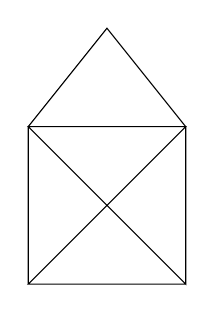
\begin{tikzpicture}
\draw (0,0) -- (0,2) -- (1,3.25) -- (2,2) -- (2,0) -- (0,2) -- (2,2) -- (0,0) -- (2,0);
\end{tikzpicture}
    
	\caption[Mit Tikz programmierte Grafik.]{Mit Tikz programmierte Grafik.}
	\label{fig:tikz_house}
\end{figure}

Ein etwas umfangreicheres Beispiel zur Digitaltechnik ist in Abbildung~\ref{fig:tikz_digital} dargestellt:

\begin{figure}[hbt]
	\centering
	\usetikzlibrary{circuits.logic.US,circuits.logic.IEC}
      \begin{tikzpicture}[circuit logic US]
      \matrix[column sep=7mm]
      {
      \node (i0) {0}; & & \\
      & \node [and gate] (a1) {}; & \\
      \node (i1) {0}; & & \node [or gate] (o) {};\\
      & \node [nand gate] (a2) {}; & \\
      \node (i2) {1}; & & \\
      };
      \draw (i0.east) -- ++(right:3mm) |- (a1.input 1);
      \draw (i1.east) -- ++(right:3mm) |- (a1.input 2);
      \draw (i1.east) -- ++(right:3mm) |- (a2.input 1);
      \draw (i2.east) -- ++(right:3mm) |- (a2.input 2);
      \draw (a1.output) -- ++(right:3mm) |- (o.input 1);
      \draw (a2.output) -- ++(right:3mm) |- (o.input 2);
      \draw (o.output) -- ++(right:3mm) node [right] {$y$ \quad Hier könnte Ihre Formel $y=(0 \land 0) \lor \overline{( 0 \land 1)}$ stehen};
 \end{tikzpicture}

	\caption[Mit Tikz programmierte Grafik, welche bereits vorgefertigte Bibliotheken für Symbole aus der Digitaltechnik nutzt.]{Mit Tikz programmierte Grafik, welche bereits vorgefertigte Bibliotheken für Symbole aus der Digitaltechnik nutzt.}
	\label{fig:tikz_digital}
\end{figure}

\clearpage

In der Tikz-Umgebung können auch Diagramme mit dem \textit{pgfplot}-Befehlssatz erzeugt werden. In Abbildung \ref{fig:pgfplot} sehen Sie ein Beispiel.

\begin{figure}[hbt]
	\centering
	\begin{tikzpicture}
		\begin{axis}[scale=1.3,legend entries={Messwerte mit Fehlerbalken,
			$\pgfmathprintnumber{\pgfplotstableregressiona} \cdot x  
			\pgfmathprintnumber[print sign]{\pgfplotstableregressionb}$}, legend style={draw=none},legend style={at={(0.01,0.98)},anchor=north west},xlabel=Stromstärke $I \; \mathrm{ \lbrack mA \rbrack}$,ylabel=Spannung $U \; \mathrm{ \lbrack V \rbrack}$]
		\addlegendimage{mark=*,blue}
		\addlegendimage{no markers,red}
\addplot+[error bars/.cd, y dir=both,y explicit]
table[x=x,y=y,y error=errory] 
{pgfplot/messdaten_mitfehler.dat};
\addplot table[mark=none,y={create col/linear regression={y=y}}]
{pgfplot/messdaten_mitfehler.dat};
	\end{axis}
\end{tikzpicture}
	\caption[Diagramm, erstellt mit dem \textit{pgfplot}-Befehlssatz.]{Ein Diagramm, erstellt in der \textit{tikzpicture}-Umgebung mit dem \textit{pgfplot}-Befehlssatz. Das Diagramm stellt Messdaten, deren Fehlerbalken und eine Regressionskurve dar. Die Messdaten werden von einer separaten Datei eingelesen und die Regressionskurve wurde mit \textit{pgfplot} berechnet und erstellt.}
	\label{fig:pgfplot}
\end{figure}

\clearpage

Auch hierzu der Quellcode in Listing~\ref{lst:pgfplot}.

\begin{lstlisting}[caption=Quellcode der Abbildung~\ref{fig:pgfplot}.,label=lst:pgfplot]
\begin{figure}[hbt]
\centering
\begin{tikzpicture}
		\begin{axis}[scale=1.3,legend entries={Messwerte mit Fehlerbalken,
			$\pgfmathprintnumber{\pgfplotstableregressiona} \cdot x  
			\pgfmathprintnumber[print sign]{\pgfplotstableregressionb}$}, legend style={draw=none},legend style={at={(0.01,0.98)},anchor=north west},xlabel=Stromstärke $I \; \mathrm{ \lbrack mA \rbrack}$,ylabel=Spannung $U \; \mathrm{ \lbrack V \rbrack}$]
		\addlegendimage{mark=*,blue}
		\addlegendimage{no markers,red}
\addplot+[error bars/.cd, y dir=both,y explicit]
table[x=x,y=y,y error=errory] 
{pgfplot/messdaten_mitfehler.dat};
\addplot table[mark=none,y={create col/linear regression={y=y}}]
{pgfplot/messdaten_mitfehler.dat};
	\end{axis}
\end{tikzpicture}
\caption[Diagramm, erstellt mit dem \textit{pgfplot}-Befehlssatz.]{Ein Diagramm, erstellt in der \textit{tikzpicture}-Umgebung mit dem \textit{pgfplot}-Befehlssatz. Das Diagramm stellt Messdaten, deren Fehlerbalken und eine Regressionskurve dar. Die Messdaten werden von einer separaten Datei eingelesen und die Regressionskurve wurde mit \textit{pgfplot} berechnet und erstellt.}
\label{fig:pgfplot}
\end{figure}
\end{lstlisting}

In Listing~\ref{lst:tikz} ist der Quellcode der Datei \textit{mess\_fehlerbalken.tex} dargestellt.

\begin{lstlisting}[caption=Quellcode der Datei \textit{mess\_fehlerbalken.tex}.,label=lst:tikz]
\begin{tikzpicture}
\begin{axis}[scale=1.3,legend entries={Messwerte mit Fehlerbalken,
$\pgfmathprintnumber{\pgfplotstableregressiona} \cdot x  
\pgfmathprintnumber[print sign]{\pgfplotstableregressionb}$}, legend style={draw=none},legend style={at={(0.01,0.98)},anchor=north west},xlabel=Stromstärke $I \; \mathrm{ \lbrack mA \rbrack}$,ylabel=Spannung $U \; \mathrm{ \lbrack V \rbrack}$]
\addlegendimage{mark=*,blue}
\addlegendimage{no markers,red}
\addplot+[error bars/.cd, y dir=both,y explicit]
table[x=x,y=y,y error=errory] 
{pgfplot/messdaten_mitfehler.dat};
\addplot table[mark=none,y={create col/linear regression={y=y}}]
{pgfplot/messdaten_mitfehler.dat};
\end{axis}
\end{tikzpicture}
\end{lstlisting}

\clearpage

In Abbildung~\ref{fig:pgfplot2y} wird ein weiters Beispiel für ein Diagramm gezeigt. Oftmals wird eine zweite y-Achse verwendet, um verschiedene Skalen darstellen zu können.

\begin{figure}[hbt]
	\centering
	\begin{tikzpicture}
%
\begin{axis}[
scale=1.3,
ytick pos=left,
xlabel=Zeit $t \; \mathrm{ \lbrack ns \rbrack}$,
ylabel=Spannung $U \; \mathrm{ \lbrack V \rbrack}$
]
\addplot[mark=*,only marks] table[x=x,y=y1] {pgfplot/messdaten_zweiyachsen.dat};
\end{axis}
%
\begin{axis}[
scale = 1.3,
legend style={draw=none},
legend style={at={(0.75,0.6)},
anchor=north west},
axis y line*=right,
axis x line=none,
%ymin=0,
%ymax=100,
ylabel=Strom $I \; \mathrm{ \lbrack mA \rbrack}$
]
\addlegendimage{mark=*,only marks}
\addlegendentry{Spannung}
\addplot[mark=x,only marks,blue] table[x=x,y=y2] {pgfplot/messdaten_zweiyachsen.dat};
\addlegendentry{Strom}
\end{axis}
\end{tikzpicture}
	\caption[Diagramm mit zwei unterschiedlichen y-Achsen.]{Diagramm mit zwei unterschiedlichen y-Achsen.}
	\label{fig:pgfplot2y}
\end{figure}

\clearpage

\subsection{Tabellen}

\begin{table}[hbt]	
	\centering
	\renewcommand{\arraystretch}{1.5}	% Skaliert die Zeilenhöhe der Tabelle
	\captionabove[Liste der verwendeten Messgeräte]{Liste der verwendeten Messgeräte. Die Genauigkeitsangaben beziehen sich auf die Standardabweichung $1\cdot \sigma$.}
	\label{tab:bsp}
	\begin{tabular}{ccccc}
		\textbf{Messgerät} & \textbf{Hersteller} & \textbf{Typ} & \textbf{Verwendung} & \textbf{Genauigkeit}\\ 
		\hline 
		\hline 
		\parbox[t]{0.2\linewidth}{\centering Spannungs-\\versorgung} & Voltmaker & HV2000 & \parbox[t]{0.2\linewidth}{\centering Spannungs-\\versorgung der\\Platine} & $\Delta U = \pm 5 $~mV \\ % Der parbox-Befehl ist erforderlich, damit ein Zeilenumbruch erzeugt werden kann. c-Spalten (zentriert) erlauben nicht automatisch einen Zeilenumpruch. Linksbündig gesetzte p-Spalten erlauben automatisch den Zeilenumbruch.
		Strommessgerät & Currentcount & Hotamp 16 & \parbox[t]{0.2\linewidth}{ \centering Strommessung\\am Versorgungspin\\des µC} & $\Delta I = \pm 0.1$~A \\ 
		\hline 
	\end{tabular} 
\end{table}

Der Quellcode der Beispieltabelle~\ref{tab:bsp} ist in Listing~\ref{lst:tab} zu sehen.

\begin{lstlisting}[caption=Quellcode der Tabelle~\ref{tab:bsp}.,label=lst:tab]
\begin{table}[hbt]	
\centering
\renewcommand{\arraystretch}{1.5}	% Skaliert die Zeilenhöhe der Tabelle
\captionabove[Liste der verwendeten Messgeräte]{Liste der verwendeten Messgeräte. Die Genauigkeitsangaben beziehen sich auf die Standardabweichung $1\cdot \sigma$.}
\label{tab:bsp}
\begin{tabular}{ccccc}
\textbf{Messgerät} & \textbf{Hersteller} & \textbf{Typ} & \textbf{Verwendung} & \textbf{Genauigkeit}\\ 
\hline 
\hline 
\parbox[t]{0.2\linewidth}{\centering Spannungs-\\versorgung} & Voltmaker & HV2000 & \parbox[t]{0.2\linewidth}{\centering Spannungs-\\versorgung der\\Platine} & $\Delta U = \pm 5 $~mV \\ % Der parbox-Befehl ist erforderlich, damit ein Zeilenumbruch erzeugt werden kann. c-Spalten (zentriert) erlauben nicht automatisch einen Zeilenumpruch. Linksbündig gesetzte p-Spalten erlauben automatisch den Zeilenumbruch.
Strommessgerät & Currentcount & Hotamp 16 & \parbox[t]{0.2\linewidth}{ \centering Strommessung\\ am Versorgungspin\\ des \textmu C} & $\Delta I = \pm 0.1$~A \\ 
\hline 
\end{tabular} 
\end{table}
\end{lstlisting}

\clearpage

\subsection{Formeln}

Formeln lassen sich in \LaTeX~ganz einfach schreiben. Es gibt unterschiedliche Umgebungen zum Schreiben von Formeln. Z.B. direkt im Text $v=s/t$ oder abgesetzt

\[F=m \cdot a\]

oder auch, wie in wissenschaftlichen Dokumenten üblich, nummeriert

\begin{equation}
P=\frac{U^2}{R} \quad .
\label{eqn:leistung}
\end{equation}

Mit einem Label in Formel~\ref{eqn:leistung} lassen sich natürlich auch Formeln im Text referenzieren. \LaTeX~verwendet im Formelmodus einen eigenen Schriftsatz, welcher entsprechend der gängigen Konventionen kursive Zeichen verwendet. Sollen im Formelmodus Einheiten in normaler Schriftart eingefügt werden, dann kann dies über den Befehl \textbackslash \textit{mathrm}\{\} erwirkt werden, wie im Quellcode von Formel~\ref{eqn:leistungMitEinh} zu sehen ist.

\begin{equation}
P=\frac{U^2}{R} = \frac{\left( 100~\mathrm{V}\right)^2}{100~\Omega} = 100~\mathrm{W}\quad .
\label{eqn:leistungMitEinh}
\end{equation}

Zum direkten Vergleich sind die Einheiten in Formel~\ref{eqn:leistungMitEinhfalsch} falsch dargestellt:

\begin{equation}
P=\frac{U^2}{R} = \frac{\left( 100~V\right)^2}{100\,\varOmega} = 100\,W
\label{eqn:leistungMitEinhfalsch}
\end{equation}

Zur einfachen Eingabe von Einheiten kann auch das Package \textbackslash \textit{siunitx} verwendet werden:

\begin{equation}
	P=\SI{100}{\watt}=\SI{100}{\joule\per\second}
\end{equation}

Das sind nur ein paar wenige Beispiele und es gibt sehr viele Packages, um Besonderheiten in Formeln realisieren zu können, z.B. mehrzeilige Formeln mit vertikaler Ausrichtung. Nennen Sie Formeln nur, wenn diese zum besseren Verständnis auch wirklich nützlich sind.

Folgende Befehle sind innerhalb von Formel-Umgebungen nützlich:
\begin{tabbing}
	\hspace*{0cm} \= \hspace{0.35\linewidth} \= \+\kill
	\textbackslash \textit{text}\{\}	\> Damit kann in Formel-Umgebung Text geschrieben werden.\\ 
	\textbackslash, \textbackslash: \textbackslash; oder \textbackslash quad und \textbackslash qquad \> Zusätzlichen Abstand zwischen Symbolen einfügen.\\
	\textbackslash \textit{notag} \> Nummerierung einer bestimmten Formel ausschalten.
\end{tabbing}

Abschließend nochmals ein kleines Beispiel:

\begin{eqnarray}
\sum\limits_{n=1}^\infty f\left(x_n\right)\cdot \Delta x=  \lim\limits_{\Delta x \rightarrow 0} \frac{f\left(x_0+\Delta x\right)-f\left(x_0\right)}{\Delta x} = \frac{\diff f}{\diff x} = \dot{f}(x)
\end{eqnarray}		% Zeile auskommentieren bei finalem Dokument!
\end{document}